\clearpage
\appendix
\section*{Supplementary material}
\section{Additional results}
\label{app:more}
Counterfactual probes (Table~\ref{tab:cf}), per-identity metrics (Table~\ref{tab:identity}), heuristic error tags
(Table~\ref{tab:tags}), risk-coverage (Figure~\ref{fig:rc}), and per-identity FPR and template scores
(Figure~\ref{fig:templates}).

\begin{table}[t]\centering\small\setlength\tabcolsep{3pt}
\resizebox{\linewidth}{!}{\begin{tabular}{lccccc}\toprule
& \multicolumn{3}{c}{Template spread $\downarrow$} & Real & Neutral\\
Model & all & seen & held-out & $|\Delta p|$ $\downarrow$ & flagged $\downarrow$\\\midrule
B2 ERM & 0.133 & 0.148 & 0.020 & 0.041 & 20\%\\
\quad ERM, 80K subsample & 0.101 & 0.114 & 0.029 & 0.037 & 19\%\\
\quad + reweight & 0.155 & 0.173 & 0.080 & 0.047 & 12\%\\
\quad + CDA & 0.135 & 0.109 & 0.031 & 0.011 & 27\%\\
\quad + soft labels & 0.108 & 0.118 & 0.026 & 0.036 & 15\%\\
\quad + combo & 0.108 & 0.094 & 0.041 & 0.009 & 19\%\\
\midrule
bert-mini ERM (80K, CPU) & 0.123 & 0.125 & 0.114 & 0.035 & 26\%\\
\quad + reweight & 0.125 & 0.135 & 0.096 & 0.032 & 8\%\\
\quad + CDA & 0.088 & 0.086 & 0.072 & 0.015 & 27\%\\
\quad + group DRO & 0.101 & 0.101 & 0.093 & 0.030 & 1\%\\
\quad + soft labels & 0.080 & 0.079 & 0.079 & 0.027 & 15\%\\
\quad + combo & 0.096 & 0.100 & 0.073 & 0.013 & 11\%\\
\midrule
B3 DistilBERT ERM & 0.114 & 0.122 & 0.088 & 0.038 & 19\%\\
\quad + reweight & 0.109 & 0.116 & 0.090 & 0.037 & 3\%\\
\quad + CDA & 0.101 & 0.094 & 0.094 & 0.012 & 21\%\\
\quad + group DRO & 0.126 & 0.123 & 0.121 & 0.033 & 0\%\\
\quad + soft labels & 0.081 & 0.095 & 0.036 & 0.033 & 16\%\\
\quad + combo & 0.112 & 0.109 & 0.103 & 0.009 & 12\%\\
\bottomrule\end{tabular}}
\caption{Counterfactual probes. \emph{Template spread}: mean absolute deviation of $P(\text{toxic})$ from the template mean across 18 identity terms (8 neutral and 5 toxic templates), split into terms in the CDA lexicon (\emph{seen}) and 5 held-out terms (sikh, queer, arab, mexican, african american). \emph{Real}: mean $|p(\text{swap})-p(\text{original})|$ over in-category swaps of 2{,}000 test comments. \emph{Neutral flagged}: share of the 144 neutral template sentences above the model's threshold.}\label{tab:cf}
\end{table}
\begin{table}[t]\centering\small\setlength\tabcolsep{3pt}
\resizebox{\linewidth}{!}{\begin{tabular}{lcccccc}\toprule
& \multicolumn{3}{c}{bert ERM} & \multicolumn{3}{c}{best}\\
Tag & FP & FN & ok & FP & FN & ok\\\midrule
identity mention & 62\% & 61\% & 37\% & 60\% & 62\% & 37\%\\
profanity & 5\% & 4\% & 2\% & 5\% & 4\% & 2\%\\
insult word & 15\% & 9\% & 4\% & 14\% & 9\% & 4\%\\
quote or reported & 30\% & 36\% & 30\% & 30\% & 37\% & 30\%\\
sarcasm marker & 4\% & 5\% & 4\% & 4\% & 5\% & 4\%\\
borderline label & 56\% & 92\% & 14\% & 56\% & 92\% & 14\%\\
few raters ($<$6) & 24\% & 2\% & 66\% & 23\% & 2\% & 66\%\\
$n$ & 6,666 & 4,399 & 121,542 & 7,215 & 4,081 & 121,311\\
\bottomrule\end{tabular}}
\caption{Share of test comments carrying each heuristic tag, by outcome. \emph{borderline label}: 30--70\% of raters said toxic.}\label{tab:tags}
\end{table}
\begin{table*}[t]\centering\small
\resizebox{\linewidth}{!}{\begin{tabular}{lrrccccccccc}\toprule
& & & \multicolumn{3}{c}{BPSN AUC $\uparrow$} & \multicolumn{3}{c}{FPR $\downarrow$} & \multicolumn{3}{c}{FNR $\downarrow$}\\
Identity & $n$ & toxic & TF-IDF & ERM & best & TF-IDF & ERM & best & TF-IDF & ERM & best\\\midrule
LGBTQ & 4,390 & 27\% & 0.783 & 0.829 & 0.838 & 0.200 & 0.204 & 0.204 & 0.352 & 0.273 & 0.272\\
black & 4,826 & 31\% & 0.721 & 0.798 & 0.821 & 0.277 & 0.242 & 0.234 & 0.287 & 0.247 & 0.247\\
christian & 13,277 & 9\% & 0.925 & 0.947 & 0.947 & 0.048 & 0.046 & 0.050 & 0.491 & 0.386 & 0.359\\
female & 16,309 & 14\% & 0.886 & 0.923 & 0.929 & 0.072 & 0.071 & 0.074 & 0.403 & 0.328 & 0.315\\
male & 14,185 & 15\% & 0.873 & 0.913 & 0.919 & 0.085 & 0.086 & 0.091 & 0.375 & 0.308 & 0.290\\
muslim & 6,861 & 23\% & 0.798 & 0.861 & 0.870 & 0.163 & 0.141 & 0.145 & 0.388 & 0.332 & 0.327\\
other religions & 3,454 & 15\% & 0.863 & 0.908 & 0.910 & 0.101 & 0.084 & 0.095 & 0.395 & 0.386 & 0.353\\
white & 7,828 & 28\% & 0.733 & 0.812 & 0.824 & 0.250 & 0.208 & 0.220 & 0.284 & 0.274 & 0.261\\
\bottomrule\end{tabular}}
\caption{Per-identity test metrics for TF-IDF ERM, DistilBERT ERM, and the best mitigated DistilBERT model by validation bias AUC (\texttt{bert\_distil\_soft}). BPSN AUC is low when non-toxic comments that mention the group score above toxic comments that don't.}\label{tab:identity}
\end{table*}
\begin{figure}[t]\centering
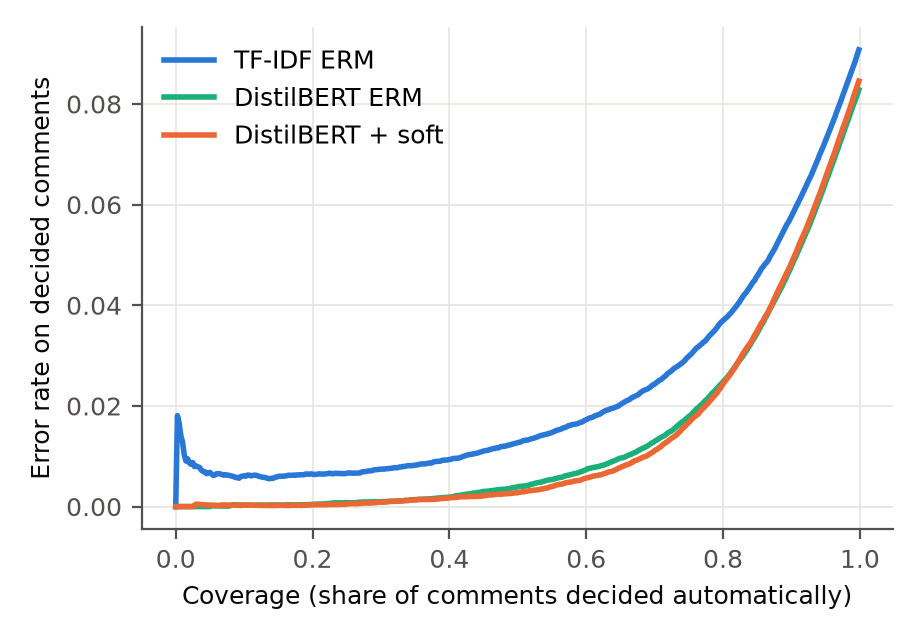
\includegraphics[width=\columnwidth]{../results/fig_risk_coverage.png}
\caption{Risk-coverage on test: error rate among the comments decided automatically, when the least confident are
deferred first. Confidence is the logit distance from each model's validation threshold.}\label{fig:rc}
\end{figure}
\begin{figure*}[t]\centering
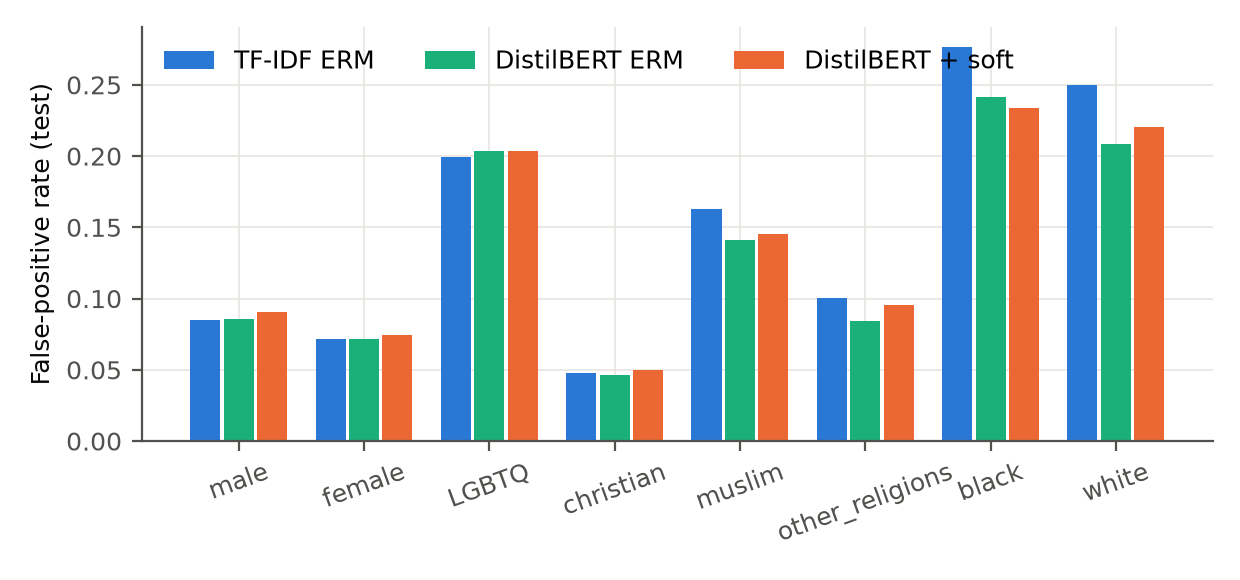
\includegraphics[width=0.49\textwidth]{../results/fig_fpr_by_identity.png}\hfill
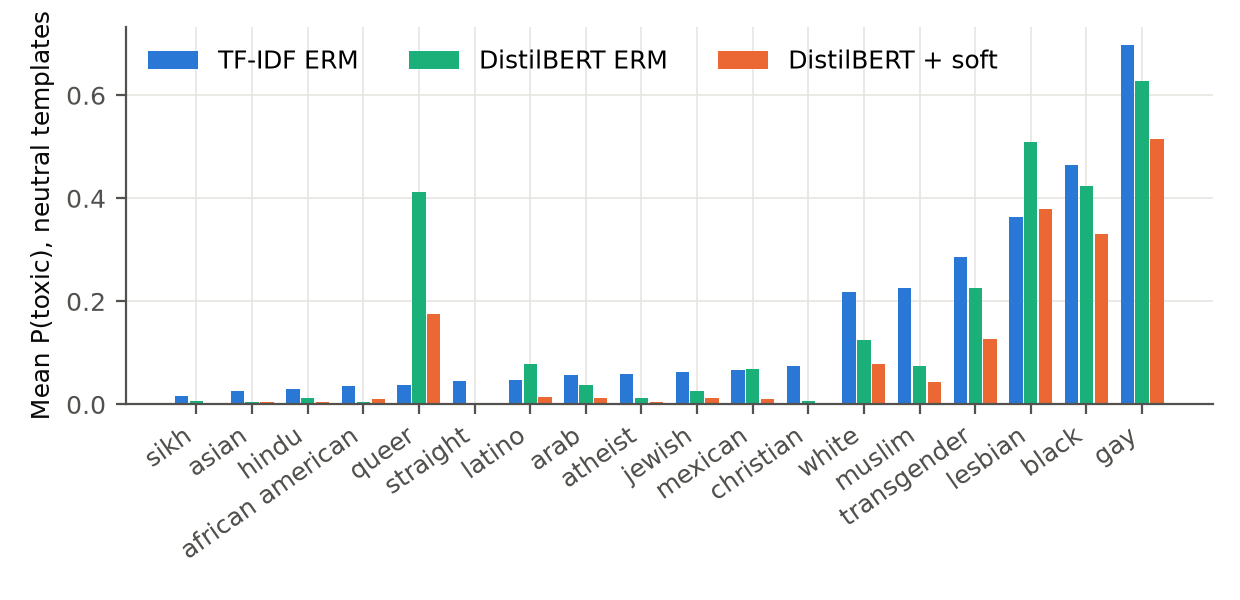
\includegraphics[width=0.49\textwidth]{../results/fig_templates.png}
\caption{Left: test FPR by identity. Right: mean $P(\text{toxic})$ on neutral template sentences by identity term,
sorted by TF-IDF ERM. The ERM models' worst FPRs are on \emph{black}, \emph{white}, \emph{LGBTQ}, and
\emph{muslim}.}\label{fig:templates}
\end{figure*}

\onecolumn
\section{Changes from the proposal}
\label{app:changes}
\begin{center}\small
\begin{tabular}{p{0.24\textwidth}p{0.30\textwidth}p{0.38\textwidth}}\toprule
Proposal & Final & Why \\\midrule
Training on university GPU servers & DistilBERT on the Dartmouth Discovery cluster (free-tier \texttt{gpu\_preempt}: H200, A5000/A5500, RTX 2080 Ti); bert-mini on a 12-core laptop CPU & As proposed for B3. Jobs stream code and data over \texttt{srun} stdin/stdout because GPU nodes cannot read home storage. The CPU runs are kept as a compute-constrained comparison (bert-mini ${\sim}150$, bert-small ${\sim}18$, DistilBERT ${\sim}7$ train examples/s on the laptop). \\
DistilBERT or RoBERTa-base (B3) & DistilBERT, full 267K training split, 1 epoch; plus bert-mini on an 80K subsample & DistilBERT matches the proposal. RoBERTa-base was not run. A same-subsample TF-IDF run (\texttt{erm80k}) separates data size from model family. \\
Three seeds for neural models & Three seeds for every DistilBERT variant; one for bert-mini & DistilBERT seeds are cheap on the cluster. bert-mini runs took ${\sim}40$ CPU-minutes each, so its comparisons rest on bootstrap CIs, which cover test sampling only. \\
Soft labels from the 1.8M Hugging Face pool & Soft labels joined by comment id from the WILDS raw file & Same annotator fractions without the cross-release leakage risk (90.5\% text overlap). The 1.8M pool is unused. \\
Truncate at 256 subword tokens & 128 wordpieces for every transformer & Fixed for the CPU bert-mini runs and kept for DistilBERT so the families share one recipe. It truncates \TokOverOneTwoEight{} of test comments, against \TokOverTwoFiveSix{} at 256; one hand-coded missed slur sits past the cut (Section~\ref{sec:errors}). \\
Captum for integrated gradients & 20-line hand-written IG with a completeness self-check & Avoids a dependency; the completeness axiom is checked numerically. \\
Group DRO on both model families & transformers only & DRO needs a per-batch loss loop; sklearn's logistic regression has none. \\
200 hand-coded errors & 200 hand-coded errors of the best model, 100 FP and 100 FN (\texttt{results/}\allowbreak\texttt{errors\_hand\_coded.csv}), plus heuristic tags on all errors & As proposed. The hand labels are the author's own; the automated tags extend coverage to every error and are checked against the hand labels (Section~\ref{sec:errors}). \\
\bottomrule\end{tabular}
\end{center}

\section{Settings}
\label{app:settings}
\begin{center}\small
\begin{tabular}{lp{0.74\textwidth}}\toprule
TF-IDF & word 1--2 grams, min\_df 3, 300{,}000 features, sublinear tf; vectoriser fit once on the training split \\
Logistic regression & L2, $C{=}4$, liblinear, max\_iter 300 \\
DistilBERT & \texttt{distilbert-base-uncased}, 7 sigmoid heads, mean BCE, lr $5{\times}10^{-5}$, bf16 autocast where supported, full training split \\
bert-mini & \texttt{prajjwal1/bert-mini}, tokenizer \texttt{bert-base-uncased}, same heads, lr $10^{-4}$, CPU \\
Optimisation & AdamW, weight decay 0.01, batch 32, 1 epoch, 6\% linear warm-up then linear decay, grad-norm clip 1.0 \\
Sequence length & 128 wordpieces, dynamic padding, length-bucketed shuffled batches \\
Training data & DistilBERT: all 267{,}112 training comments. bert-mini: 80{,}000 sampled with seed 0 (same sample for every variant). CDA adds copies \\
Reweighting & inverse frequency of 18 groups, normalised to mean 1, clipped at 10 \\
Group DRO & online exponentiated gradient over 18 groups, $\eta{=}0.01$ \\
Calibration & one temperature on the toxicity logit, grid over $[0.25, 4]$, minimum validation NLL \\
Threshold & validation-F1-optimal over $\{0.05, 0.06, \dots, 0.95\}$ \\
IG & [PAD]-embedding baseline, special tokens fixed, 48 steps (32 in the error analysis) \\
Bootstrap & 50 test-set resamples, percentile 95\% interval \\
Seeds & data subsample fixed at 0; training seed 0 (all models) and 1, 2 (DistilBERT) \\
\bottomrule\end{tabular}
\end{center}
